\chapter{Simulation}

The frontend can be quite interesting as just a way to survey a city from a bird's eye view. The program's real use lies in data analysis, though. Over the semester, I tried multiple approaches for creating an agent-based simulation, with all but the last attempt failing due to technical circumstances.

\section{Deprecated versions}

The first concept was very simple. Each agent would pick a two random buildings as start and end points, and would travel between them in a straight line, with constant speed. Actors would be shown in the graphical scene as individual cubes, moving in small increments. The backend simulated movement in one minute steps, and after each one, the modified agents would be collected and sent over the websocket in multiple chunks, so as to reduce the chances of overloading the socket. The problem here was one of scalability. Fifty or a hundred agents could easily be processed and shown in real time, but that obviously was not enough to draw any meaningful conclusions about behaviour. Displaying more agents caused a simply unacceptable framerate of three frames per second. Although I used the same visual model for every agent, batching and caching could not be used due to the chaotic nature of their overall movement. The design is visible in the appendix, at~\ref{overlay_v1}

The second version improved performance by processing the agent updates non-visually and dividing up the playfield into relatively small chunks to act as a heatmap; it was a separately renderable on top of the main scene. Each update's coordinates were fed into the overlay, and an opacity value was calculated for every chunk. The result was a serviceable tool that, while updating constantly, still had bad performance. A new object cache was being created every time I opened the heatmap UI, and this taxed the rendering thread heavily. However, once all updates have been processed, the performance was decent. This gave me the idea of running full simulations as fast as possible, and only transferring the final values over the socket. This design is also in the appendix, at~\ref{overlay_v2}

\label{simulation-working}
\section{The working implementation}

I ended up keeping the agent idea, but focused on the need for the frontend to be uninvolved aside from requesting and displaying content. As such, the server only recognises its own spatial scale and the heatmap's chunk size needs to be converted. The client can choose time constraints and an agent count for the simulation, using fields in the dialog opened by the "play" button on the frontend.

The server starts each simulation from scratch by copying the HeatmapData instance sent by the client. The requested number of agents is randomly distributed on the map, with the buildings chosen from the database, weighted by the "capacity" column: a large residential building is more likely to have agents start there than a small boutique. Each person can then choose a target building every minute, but may also choose to remain where they are. With a resolution of 7.5 simulated seconds, the difference between the goal and the current location is determined, normalised, and the agent is nudged along by adding this value to its position multiplied by the agent's speed. As of now, the speed is pre-determined in the Agent class, intended as a placeholder for different vehicle types.

The simulation constantly the copied instance, adding one to the value of the cell that contains the current step. The grid size is received in degrees of latitude/longitude. The correct cell's id is calculated by flooring the coordinates using the baseline and grid size. The map is not pre-allocated, the desired cell is created on the fly if it does not exist -- this reduces data transfer significantly. Updates are grouped by minute and then by agent. Once the terminal state is reached, a SimulationResult message is sent back with the heatmap cells.

The data is transformed by the client, scaling the coordinates contained in each cell's identifier back, and placing each integer into the correct slot of the libGDX heatmap. Every value is absolute, scaling is done at render time.
\begin{figure}[h]
    \centering
    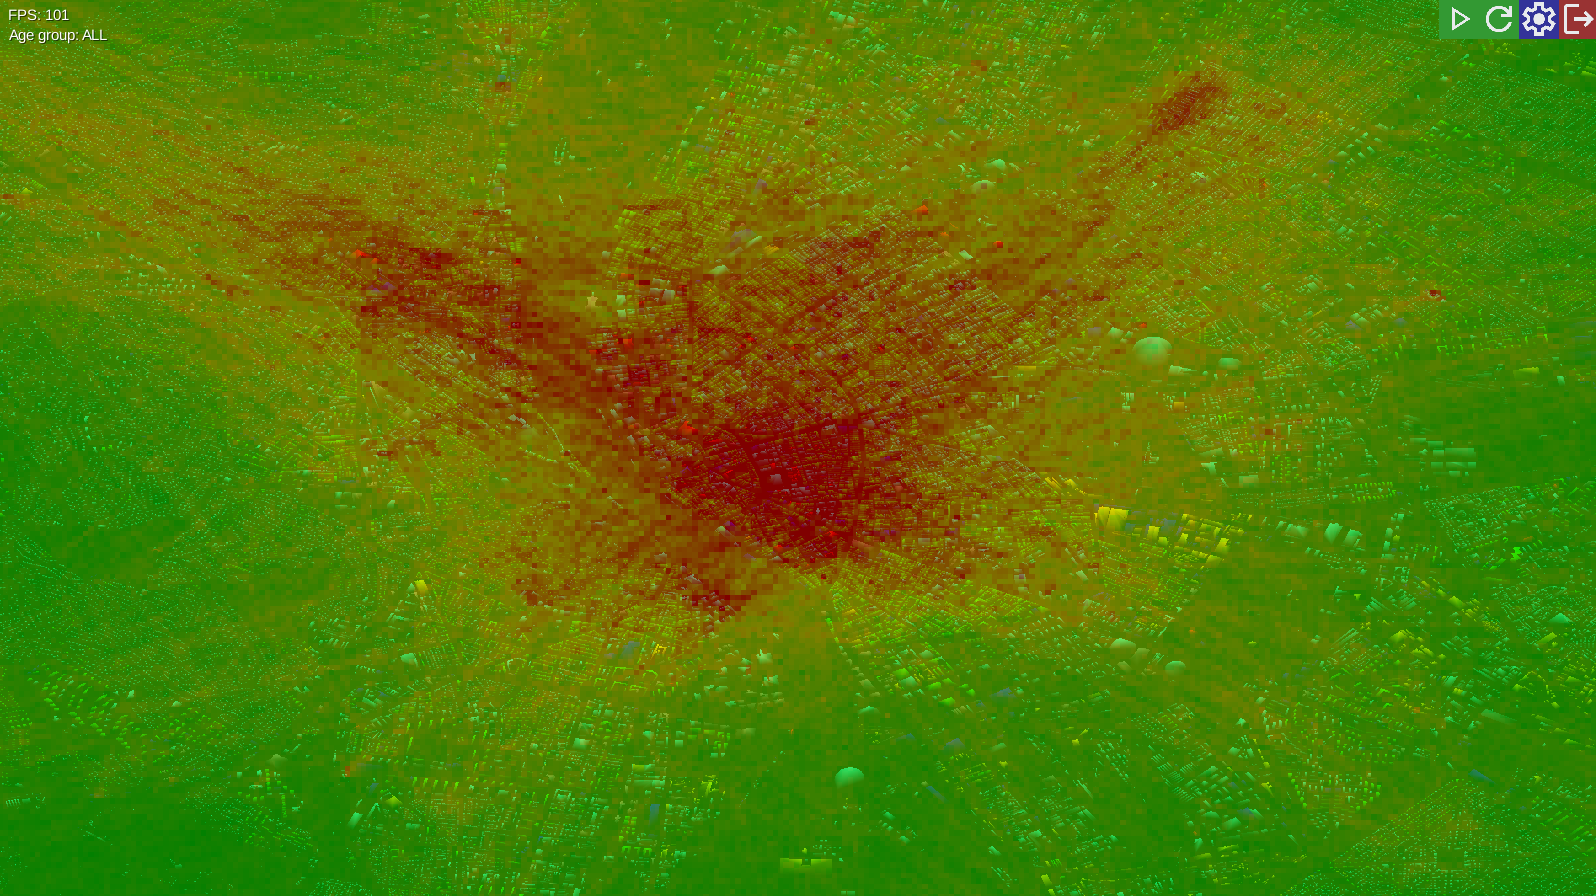
\includegraphics[width=140mm, keepaspectratio]{images/overlay_v3.png}
    \caption{A shaded overlay, showing most common agent paths; this version ended up in the program\ \label{overlay_v3}}
\end{figure}

\subsection{Building selection logic}

People in the simulation choose targets based on a simplified statistical model. They may be in one of four primary age groups: children, teens, adults or the elderly. Time of day, age group and building type can be represented as a three-dimensional distribution. Some building types (such as schools) are visited rarely at night, but very often in mornings. Age group and building type is connected as well: children are generally not expected to travel to industrial complexes.

I represented this as two static distributions, stored on the server's side. Agents first decide if they want to travel at all, this happens 25\% of the time overall, split up into two checks. The chance of a given agent travelling to a certain building type is calculated by multiplying the time-type and age-type values together. Each product is the probability of travelling to the given building type; agents pick a random type that has a chance between 0 and a randomly selected floating point value, up to 1. If the calculated building variety is the same as the current building, the agent does not leave; otherwise, a random building is picked, the likelihood of any individual target is decreases with distance. The process maintains a pool of buildings to pick from. When an item is selected, it's removed from the cache. If the cache has no buildings of the selected type, a request is made to the database for that type.

The method thus has three random variables. This requires many more agents than a more sophisticated model to achieve the expected distribution, but its accuracy is acceptable, provided the required processing power is available. Since the model is based on individual decisions, expansion is not too difficult -- more variables can be added as needed. 

I took inspiration from the video game Cities: Skylines II for the simulation system. There, pathfinding is based on time, comfort, money and individual citizen behaviour.\cite{CSII-traffic} The most important takeaway was the differing needs of certain age groups. As comfort and money was not applicable, I instead differentiated agent behaviour by the type of buildings they would visit at certain hours of the day. Travel time is a linear function of the distance covered and not influenced by road geometry. This was overall a computationally cheap and easier to implement solution, and it still provided specific patterns for the four age groups (see appendix at~\ref{age-groups}).